% Biểu mẫu D2 được đính kèm nguyên trạng. Tiêu đề mục được ghi thẳng vào mục lục
% (và neo vào trang đính kèm đầu tiên) thay vì dùng \section, vì \includepdf gọi
% \clearpage nên tiêu đề sẽ bị đẩy ra một trang riêng gần như trống.
% addtotoc tự tăng bộ đếm section và tự ghi số mục vào mục lục.
\IfFileExists{form/formD2.pdf}{
  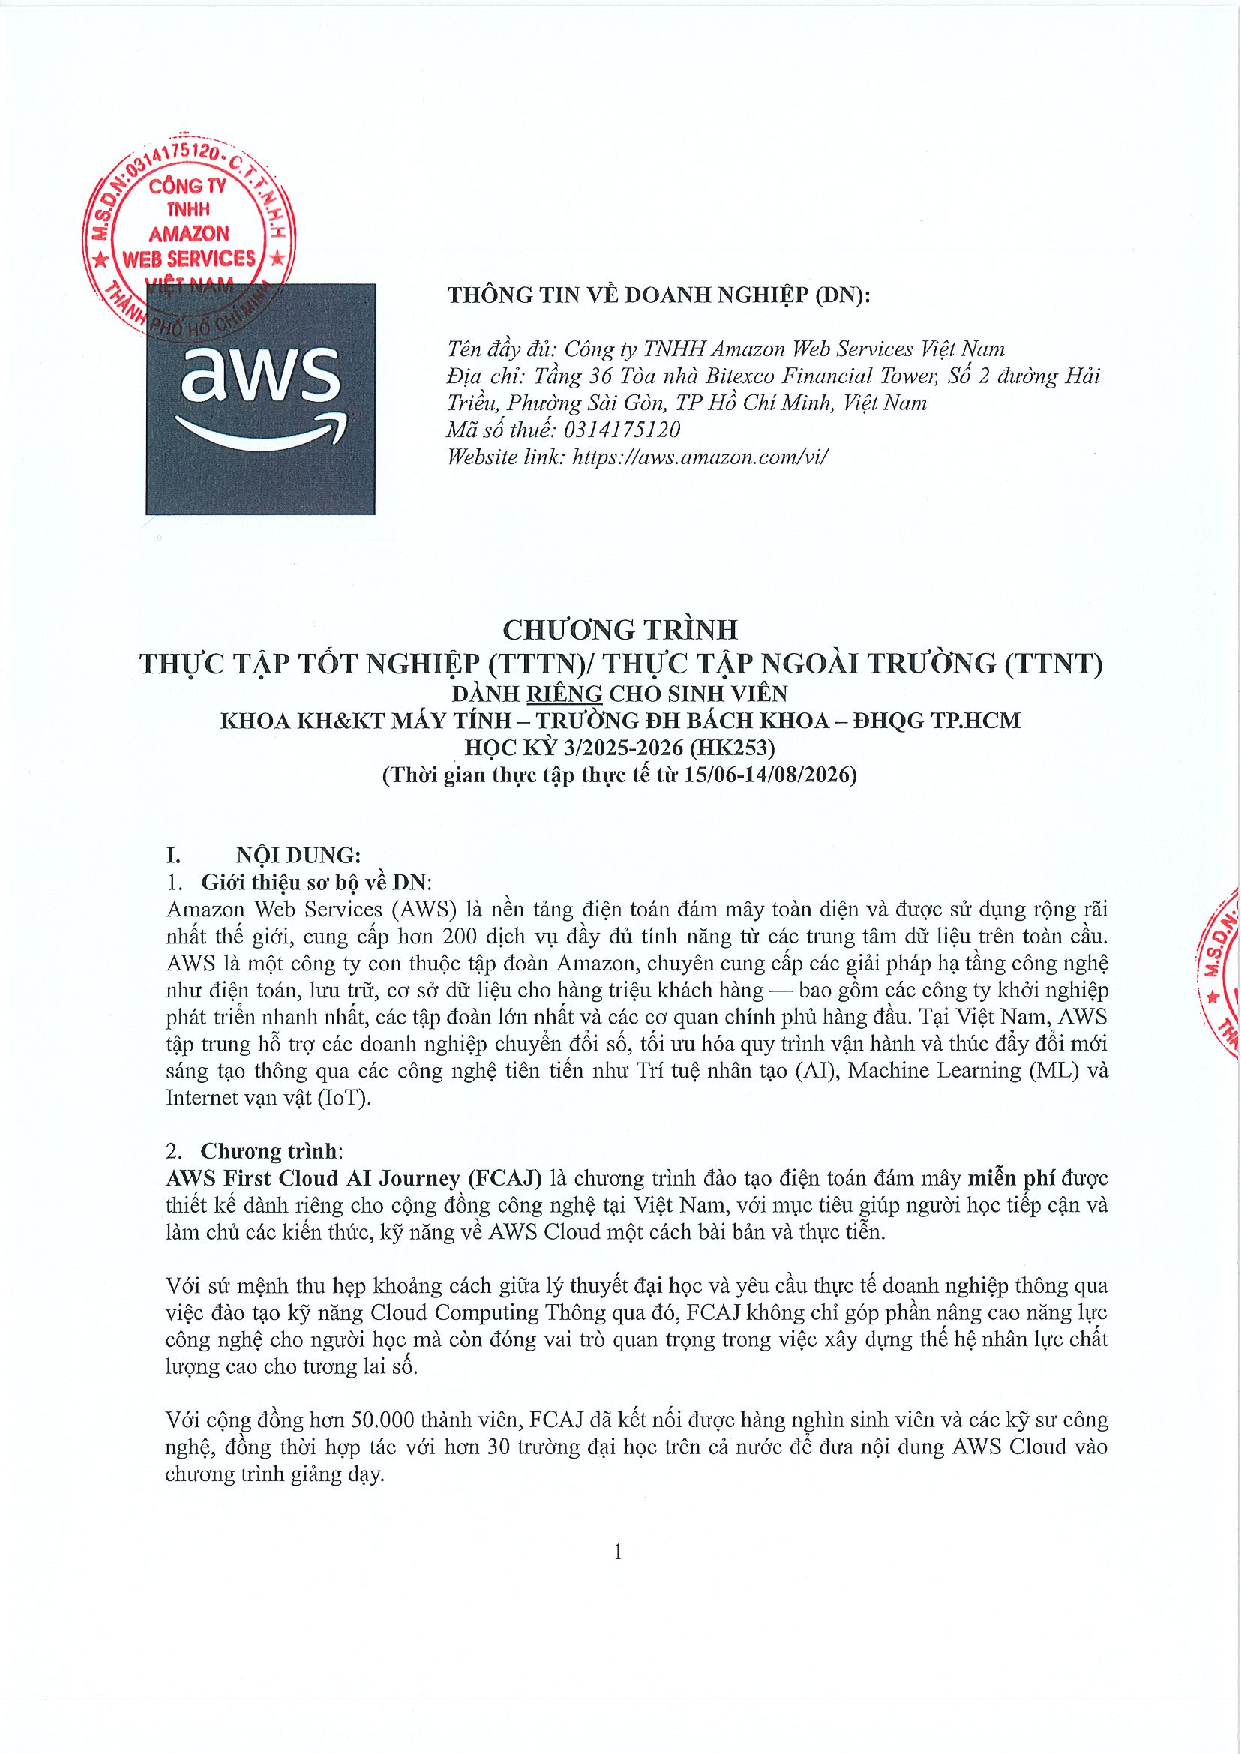
\includepdf[
    pages=-,
    addtotoc={1,section,1,Chương trình thực tập,sec:chuong-trinh-thuc-tap},
    pagecommand={\thispagestyle{empty}}
  ]{form/formD2.pdf}
}{
    \refstepcounter{section}
    \phantomsection
    \addcontentsline{toc}{section}{\protect\numberline{\thesection}Chương trình thực tập}
    \begin{center}
        \textit{Đính kèm biểu mẫu D2 tại đây}
    \end{center}
    \pagebreak
}

\endinput
